\documentclass{article}
\usepackage{amsmath}
\usepackage{amssymb}
\usepackage{graphicx}
\usepackage{hyperref}
\usepackage[version=4]{mhchem}

\title{Example 11}
\date{}

\begin{document}
\maketitle

\(A B C D\) is a convex quadrilateral. \(E\) and \(F\) are midpoints of \(A D, B C\), respectively. \(G\) and \(H\) are midpoints of diagonals \(B D, A C\), respectively. Show that \(E F\) and \(G H\) bisect each other.

Solution:
Connect the midpoints of \(E G\), and \(H F\), respectively.\\
\centering
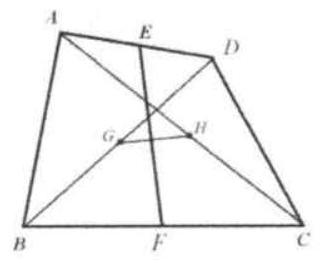
\includegraphics[width=\textwidth]{images/problem_image_1.jpg}

By Theorem 2.1, in triangle \(A B D, E G / / A B, E G=\frac{1}{2} A B\), and in triangle \(A B C, H F / / A B, H F=\frac{1}{2} A B\).\\
Thus \(E G / / H F\) and \(E G=H F\).\\
So \(E G F H\) is a parallelogram. \(E F\) and \(G H\) bisect each other.\\
\centering
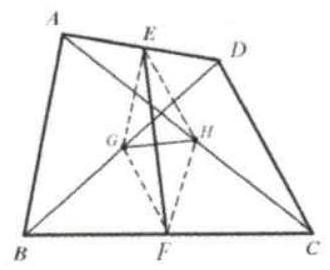
\includegraphics[width=\textwidth]{images/reasoning_image_1.jpg}


\end{document}
